\documentclass{article}
\usepackage{graphicx}
\usepackage[utf8]{inputenc}
\usepackage[T1]{fontenc}
\usepackage{imakeidx}
\usepackage{hyperref}
\usepackage{listings}
\usepackage{amsthm}

\makeindex
\hypersetup{
colorlinks,
linkcolor=blue,
urlcolor=blue,}

\title{Git for Robots}   
\author{Arjun Gandhi} 
\date{\today} 

\begin{document}


%=========================================
\begin{titlepage}
		\centering{
			{\fontsize{40}{48}\selectfont 
			Git for Robotics}
		}\\
			
		\vspace{10mm}
		\centering{\Large{Arjun Gandhi}}\\
		\vspace{\fill}
		\centering \large{March 2020}
\end{titlepage}


%=========================================
\newpage{}
\thispagestyle {empty}

\vspace*{2cm}

\begin{figure}
		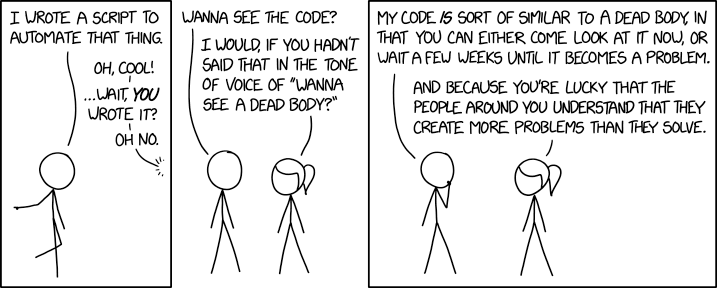
\includegraphics[width=5.5in]{images/wanna_see_the_code.png}
		\caption{This is how all of my robotics project go.}
\end{figure}

\newpage

\tableofcontents

\newpage
\section{What is version control?}

    You can think of a version control system (short: "VCS\index{version control system}") as a kind of "database". It lets you save a snapshot of your complete project at any time you want. When you later take a look at an older snapshot (let's start calling it "version\index{version}"), your VCS shows you exactly how it differed from the previous one.
    \begin{figure}[hp]
    \centering
    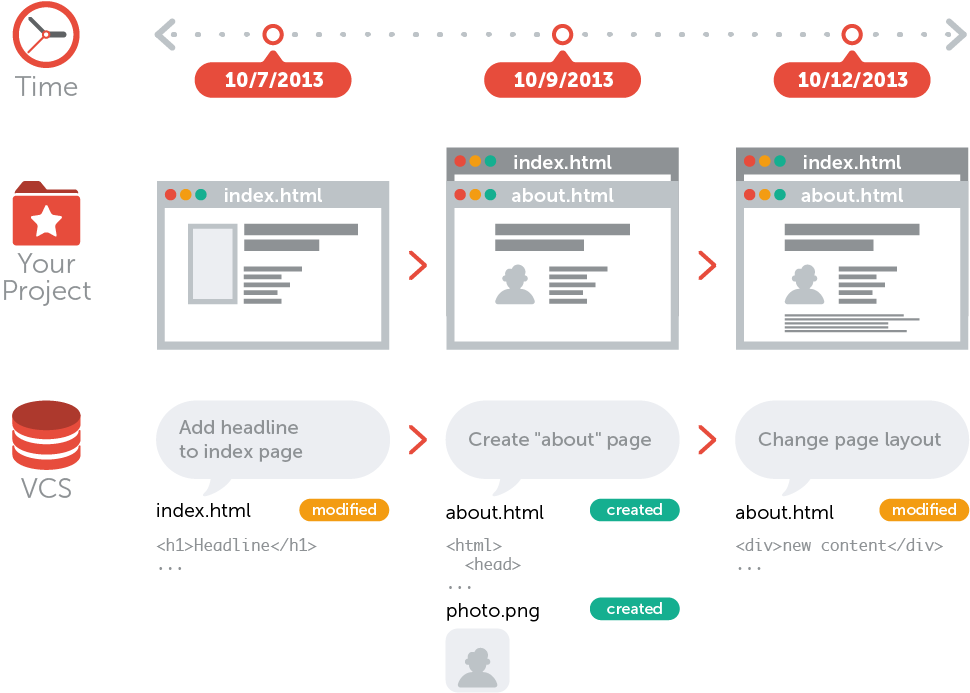
\includegraphics[width=4.5in]{images/what_is_vcs.png}
    \end{figure}
    
    Version control is independent of the kind of project / technology / framework you're working with:
    \begin{itemize}
        \item It works a website as it does for a robotics project
        \item It lets you work with any tool you like; it doesn't care what kind of text editor, graphics program, file manager or other tool you use
    \end{itemize}

    At the core of it a VCS records the changes you make to your project's files. This is what version control is about. It's really as simple as it sounds.
\subsection{Why use version control}
    
    With out a VCS you are probably working together in a shared folder on the same set of files. Texting your teammates that you are currently working on file "xyz" and that, meanwhile, your teammates should keep their fingers off. This is an awful idea. It's extremely error-prone as you're essentially doing open-heart surgery all the time: sooner or later, someone will overwrite someone else's changes.

    With a VCS, everybody on the team is able to work absolutely freely - on any file at any time. The VCS will later allow you to merge all the changes into a common version. There's no question where the latest version of a file or the whole project is. It's in a common, central place: your version control system.

    Other benefits of using a VCS are even independent of working in a team or on your own.
    
    \subsubsection{Storing Versions (Properly)}
    Making a save of your project after you make critical changes is an important and necessary habit. It prevents you from losing your new work and allows you to go back to your old work easily in case you need it. Without a VCS your save system might look like the following awful ideas (I have personally seen someone do every one of these).
    \begin{itemize}
        \item Saving the changes as a new file and appending a number/date to the end.
        \item Making a copy of the entire code and pasting it (commented out) below the actual code for each version of the code. 
        \item Copying the code and sending it in an email.
        \item Saving pictures of the code and putting them in Dropbox.
        %add more fun bad examples if you can think of it
    \end{itemize}
    The core of this however is that the problem gets out of hand fast. 
    
    A VCS solves this problem. A version control system acknowledges that there is only one project. Therefore, there's only the one version on your disk that you're currently working on. Everything else - all the past versions and variants - are neatly packed up inside the VCS. When you need it, you can request any version at any time and you'll have a snapshot of the complete project right at hand.
    \subsubsection{Restoring Old Versions}
    Being able to restore older versions of a file (or even the whole project) effectively means one thing: you can't mess up! If the changes you've made lately prove to be garbage, you can simply undo them in a few clicks. Knowing this should make you a lot more relaxed when working on important bits of a project.
    
    \subsubsection{Understanding What Changes Were Made}
    When working in large teams understanding what changes other members have done quickly is crucial to efficient working. 
    
    Every time you save a new version of your project, your VCS requires you to provide a short description of what was changed. Additionally (if it's a code / text file), you can see what exactly was changed in the file's content. This helps you understand how your project evolved between versions.
    
    \subsubsection{Backup}
    It's happened to all of us before you accidental deleted a critical file in a moment of panic. Luckily a side-effect of using a distributed VCS like Git is that it can act as a backup; every team member has a full-blown version of the project on his disk - including the project's complete history. Should your beloved central server break down (and your backup drives fail), all you need for recovery is one of your teammates' local Git repository.
    
    \subsubsection{What is Git?}
    By far, the most widely used modern version control system in the world today is Git. Git is a mature, actively maintained open source project originally developed in 2005 by Linus Torvalds, the famous creator of the Linux operating system kernel. A staggering number of software projects rely on Git for version control, including commercial projects as well as open source. Developers who have worked with Git are well represented in the pool of available software development talent and it works well on a wide range of operating systems and IDEs (Integrated Development Environments).
    
\section{Setting Up}

There are two main ways of working with Git: either via its "Command Line Interface" or with a GUI application. Neither of these are right or wrong.

On the one hand, using a GUI application is likely easier at first and can help new users with the basic features.

On the other hand, however, I recommend learning the basics of Git on the command line first. It helps you form a deeper understanding of the underlying concepts and makes you independent from any specific GUI application.

In this guide we will be using to command line interface not only because of the foundations it provides but also as it is what you will be using in the later robotics classes.

There are also several well designed third party applications, I recommend checking them out after you get a handle on git.*

*Note: Downloading a third party app is may not be supported by the RBE Department, this is due to the authentication process 


\subsection{Setting Up Git on Your Computer}

Installing Git has become incredibly easy in recent times. There are one-click installers for both Mac and Windows.

In this tutorial, like in many others, the "\$" sign represents the prompt of the command line interface (you don't have to type this character in your commands!). Therefore, any time you see a line starting with the "\$" sign, it means we're executing commands in "Terminal" or "Git Bash".


\subsubsection{Installing Git on Windows}
On Windows, you can download the "Git for Windows" package from here: \href{https://git-for-windows.github.io/}{ https://git-for-windows.github.io/}  
Allow popup: yes

When running the installer EXE, you should choose the default options in each screen. After finishing the installation, you can begin working with Git by starting the "Git Bash" application. You'll find it in the Windows START menu, inside the "Git" folder:
\begin{figure}[hp]
    \centering
    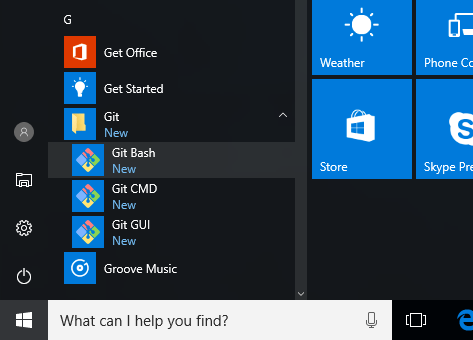
\includegraphics[width=4.5in]{images/git-bash-windows}
\end{figure}

\subsubsection{Installing Git on MacOS}

Download and run the installer from \href(https://sourceforge.net/projects/git-osx-installer/files/){here}.
Follow the prompts to install Git.

Note: if you are already using Homebrew, feel free to use that instead with the following command:
\begin{lstlisting}[language=bash]
$ brew install git
\end{lstlisting}

Then open up the terminal you can do this by starting "Terminal.app" on your Mac. You'll find this in the "Utilities" subfolder of your "Applications" folder in Finder:
\newpage
\begin{figure}[hp]
    \centering
    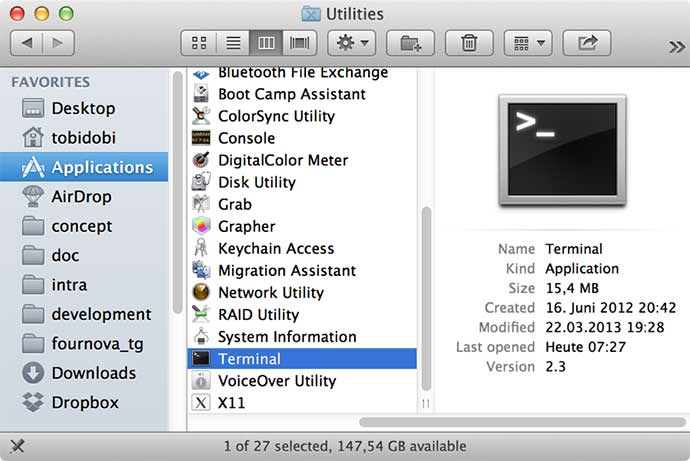
\includegraphics[width=4.5in]{images/terminal-app-mac.jpg}
\end{figure}



\subsubsection{Installing Git on Linux}
Use your the appropriate package manager for your linux system to install git:

Some of the common systems are listed below.

Open terminal and run the following commands:
\newline
\textbf{Ubuntu/Debian}

\begin{lstlisting}[language=bash]
$ sudo apt update
$ sudo apt install git
\end{lstlisting}

\textbf{Redhat Based System}
\begin{lstlisting}[language=bash]
$ sudo yum install git
\end{lstlisting}

\textbf{Arch Linux}
\begin{lstlisting}[language=bash]
$ sudo pacman -S git
\end{lstlisting}

\subsection{Setting up GitHub}

To proceed with this process you need to make a GitHub account. 

If you don't already have one you can sign up for it \href{https://github.com/join?source=header-home}{here}:

I recommend signing up for a \href{https://education.github.com/pack}{Student Developer Pack}(you get lots of free stuff)

You do need to send in a picture of your id because of WPI email addresses being weird.

\subsubsection{Configuring Git}
A couple of very basic configurations should be made before you get started. You should set your name and email address as well as enable coloring to pretty up command outputs:

Make sure to use the same email that you used for your GitHub account.

\begin{lstlisting}[language=bash]
$ git config --global user.name "John Doe"
$ git config --global user.email "john@doe.org"
$ git config --global color.ui auto
\end{lstlisting}

\section{Basic Workflow}

Before we get lost in Git commands, you should understand what a basic workflow with version control looks like. We'll walk through each step in detail later in this book. But first, let's get an understanding of what the workflow in general is like.
\newline\newline
The most basic building block of version control is a "\index{repository}repository".
\newtheorem*{repository}{Repository}
\begin{repository}
Think of a repository as a kind of database where your VCS stores all the versions and metadata that accumulate in the course of your project. In Git, the repository is just a simple hidden folder named ".git" in the root directory of your project. Knowing that this folder exists is more than enough. You don't have to (and, moreover, should not) touch anything inside this magical folder.
\end{repository}

Getting such a repository on your local machine can be done in two ways:

\begin{enumerate}
    \item If you have a project locally on your computer that is not yet under version control, you can initialize a new repository for this project.
    \item  If you're getting on board of a project that's already running, chances are there is a repository on a remote server (on the internet or on your local network). You'll then probably be provided with a URL to this repository that you will then "clone" (download / copy) to your local computer.
\end{enumerate}


(1)As soon as you have a local repository, you can start working on your files: modify, delete, add, copy, rename, or move files in whatever application (your favorite editor, a file browser, ...) you prefer. In this step, you don't have to watch out for anything. Just make any changes necessary to move your project forward.
\newline\newline
(2)It's only when you feel you've reached a noteworthy state that you have to consider version control again. Then it's time to wrap up your changes in a \index{commit}commit.
\newtheorem*{commit}{Commit}
\begin{commit}
A commit is a wrapper for a specific set of changes. The author of a commit has to comment what he did in a short "commit message". This helps other people (and himself) to understand later what his intention was when making these changes.
\newline\newline
Every set of changes implicitly creates a new, different version of your project. Therefore, every commit also marks a specific version. It's a snapshot of your complete project at that certain point in time (but saved in a much more efficient way than simply duplicating the whole project...). The commit knows exactly how all of your files and directories looked and can therefore be used, e.g., to restore the project to that certain state.
\end{commit}
(3) However, before you commit, you'll want to get an overview of what you've changed so far. In Git, you'll use the "status" command to get a list of all the changes you performed since the last commit: which files did you change? Did you create any new ones or deleted some old ones?
\newline\newline
(4) Next, you tell Git which of your local changes you want to wrap up in the next commit. Only because a file was changed doesn't mean it will be part of the next commit! Instead, you have to explicitly decide which changes you want to include. To do this, you add them to the so-called "Staging Area".
\newline\newline
(5) Now, having added some changes to the Staging Area, it's time to actually commit these changes. You'll have to add a short and meaningful message that describes what you actually did. The commit will then be recorded in your local Git repository, marking a new version of your project.
\newline\newline
(6) From time to time, you'll want to have a look at what happened in the project - especially if you're working together with other people. The "log" command lists all the commits that were saved in chronological order. This allows you to see which changes were made in detail and helps you comprehend how the project evolved.
\newline\newline
(7) Also when collaborating with others, you'll both want to share (some of) your changes with them and receive the changes they made. A remote repository on a server is used to make this exchange possible.
 
 \newtheorem*{local-remote-repos}{Local \& Remote Repositories}
 \begin{local-remote-repos}
 There are two kinds of repositories:
\newline
A "local" repository resides on your local computer, as a ".git" folder inside your project's root folder. You are the only person that can work with this repository, by committing changes to it.
A "remote" repository, in contrast, is typically located on a remote server on the internet or in your local network. No actual working files are associated with a remote repository: it has no working directory but it exclusively consists of the ".git" repository folder. Teams are using remote repositories to share \& exchange data: they serve as a common base where everybody can publish their own changes and receive changes from their teammates.
\end{local-remote-repos}

\subsection{Creating a local git repository}
\subsection{Starting with an Unversioned Project}

Let's start with an existing project that is not yet under version control. Change into the project's root folder on the command line and use the "git init" command to start versioning this project:

\begin{lstlisting}[language=bash]
$ cd path/to/project/folder
$ git init
\end{lstlisting}

Now take a moment to look at the files in that directory (including any hidden files):

\begin{lstlisting}[language=bash]
$ ls -la
\end{lstlisting}

You'll see that a new, hidden folder was added, named ".git". All that happened is that Git created an empty local repository for us. Please mind the word "empty": Git did not add the current content of your working copy as something like an "initial version". The repository contains not a single version of your project, yet.

 \newtheorem*{working-copy}{Working Copy}
 \begin{working-copy}
The root folder of your project is often called the "working copy" (or "working directory"). It's the directory on your local computer that contains your project's files.
\newline\newline
You can always ask the version control system to populate your working copy with any version of your project. But you always only have one working copy with one specific version on your disk - not multiple in parallel.
\end{working-copy}

\subsubsection{Ignoring Files}
Typically, in every project and on every platform, there are a couple of files that you don't want to be version controlled: Eclipse likes to make a massive .eclipse folder and if version controlled it has a tendancy to cause problems. In other projects, you might have build or cache files that make no sense in a version control system. You'll have to decide yourself which files you don't want to include.

 \newtheorem*{note}{Note}
 \begin{note}
What Files Should I Ignore?
\newline\newline
As a simple rule of thumb you'll most likely want to ignore files that were created automatically (as a "by-product"): temporary files, logs, cache files...
\newline\newline
Other examples for excluded files range from compiled sources to files that contain passwords or personal configurations.
\newline\newline
A helpful compilation of ignore rules for different projects and platforms can be found \href{https://www.github.com/github/gitignore}{here} 
 \end{note}

The list of files to ignore is kept in a simple file called ".gitignore" in the root folder of your project. It's highly recommended to define this list at the very beginning of your project - before making your first commit. Because once files are committed, you'll have to jump through some hoops to get them out of version control, again.
\newline\newline
Now, let's get going: Create an empty file in your favorite editor and save it as ".gitignore" in your project's root folder. If you're on a Mac, e.g., you'll want to make sure it contains at least the following line:
\newline
\begin{lstlisting}[language=bash]
.DS_Store
\end{lstlisting}

If there are other files you want to ignore, simply add a line for each one. Defining these rules can get quite complex. Therefore, to keep things simple, I'll list the most useful patterns which you can easily adapt to your own needs:
\begin{itemize}
    \item Ignore one specific file: Provide the full path to the file, seen from the root folder of your project.
    \newline
path/to/file.ext
    \item Ignore all files with a certain name (anywhere in the project): Just write down the file's name, without giving a path.
    \newline
filename.ext
    \item Ignore all files of a certain type (anywhere in the project): 
    \newline
    *.ext
    \item  Ignore all files in a certain folder:
    \newline
path/to/folder/*
\end{itemize}

\subsubsection{Making Your First Commit}
With some ignore rules in place, it's time to make our initial commit for this project. We'll go into great detail about the whole process of committing a little later in this book. For now, simply execute the following commands:

\begin{lstlisting}[language=bash]
$ git add -A
$ git commit -m "Initial commit"
\end{lstlisting}

\section{Starting with an Existing Project on a Server}

We are going to go onto github and make our first repository.
\newpage
Logon to Github and hit the new repository button:
\begin{figure}[hp]
    \centering
    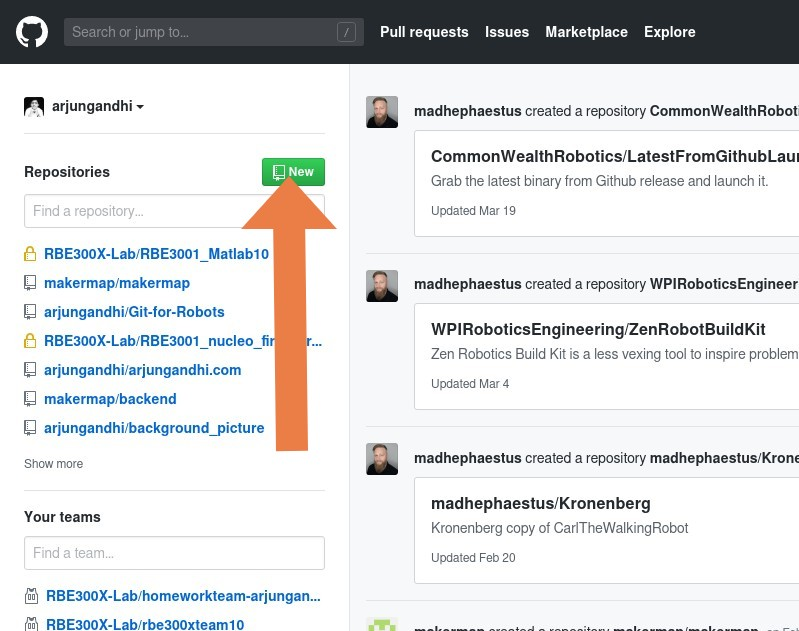
\includegraphics[width=4.5in]{images/new-repo.jpg}
\end{figure}



 \newtheorem*{temp}{Temp}
 \begin{temp}
 \end{temp}
\begin{lstlisting}[language=bash]

\end{lstlisting}


\section{Fun Stuff}
\subsection{3rd Party Git Apps}



\begin{thebibliography}{9}
\bibitem{git-tower}
A large portion of this document was "liberated" from:
https://www.git-tower.com/learn/git/ebook/en/command-line/basics/why-use-version-control
\bibitem{atlassian}
https://www.atlassian.com/git/tutorials/what-is-git
\end{thebibliography}



\end{document}
